\section{Regulation}
  Ribosome association does not necessarily imply translation
  \cite{guttman_ribosome_2013}

  Nicely described by \cite{tautz_evolutionary_2011} pp. 5.

  \subsection{General ideas}

  \subsection{Alternative splicing}

      \begin{figure}[h!]
        \centering
        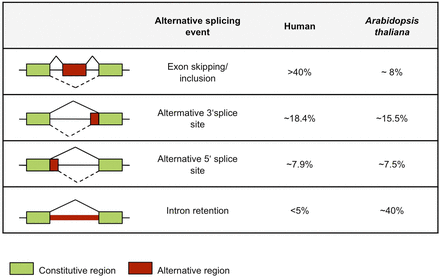
\includegraphics[width=.5\textwidth]{reddy-fig1}
        \caption{Reddy (2013) \cite{reddy_complexity_2013}}
      \end{figure}

      This may just be because Arabidopsis has such short introns. However it
      might be worth looking into how this affects orphan origins.

  \subsection{Exaption of transposon promoters}

    Many transposons are differentially regulated under stress.

    Transposon insertion into the non-exonic parts of genes may add stress
    resistence regulation or general upregulation (see Naito paper \cite{naito_unexpected_2009}).


  \subsection{Regulatory elements}

    Where do orphans get their regulatory elements? Chance?

    A nice review of plant orphans: \cite{priest_cis-regulatory_2009}.
    cis-regulatory elements coopoerate to create nuanced.

  \subsection{Papers}

    \subsubsection{Kapranov (2007) Genome-wide transcription and the
    implications for genomic organization}

      Citation \cite{kapranov_genome-wide_2007}

      A Science review on genome wide transcription 

    \subsubsection{Nagalakshmi (2008) The transcriptional landscape of the
    yeast genome defined by RNA sequencing}

      Citation \cite{nagalakshmi_transcriptional_2008}

      Yeast transciptional landscape 

      ``We applied RNA-Seq to generate a high-resolution transcriptome
      map of the yeast genome and demonstrated that most (74.5\%) of the
      nonrepetitive sequence of the yeast genome is transcribed''

    \subsubsection{Xu (2009) Bidirectional promoters generate pervasive
    transcription in yeast}
    
      Citation \cite{xu_bidirectional_2009}

    \subsubsection{Naito (2009) Unexpected consequences of a sudden and
    massive transposon amplification on rice gene expression}

      In a study by Naito (2009) \cite{naito_unexpected_2009}, the DNA
      transposon mPing was found to be proliferating in the rice strain EG4
      at a rate of about 40 jumps per generation. The TE preferentially
      jumped into genic, but not exonic, sequence. They usually upregulated
      the genes or did nothing. 156/710 showed difference in regulation, of
      these 111/156 were upregulated. 

      \begin{figure}[h!]
        \centering
        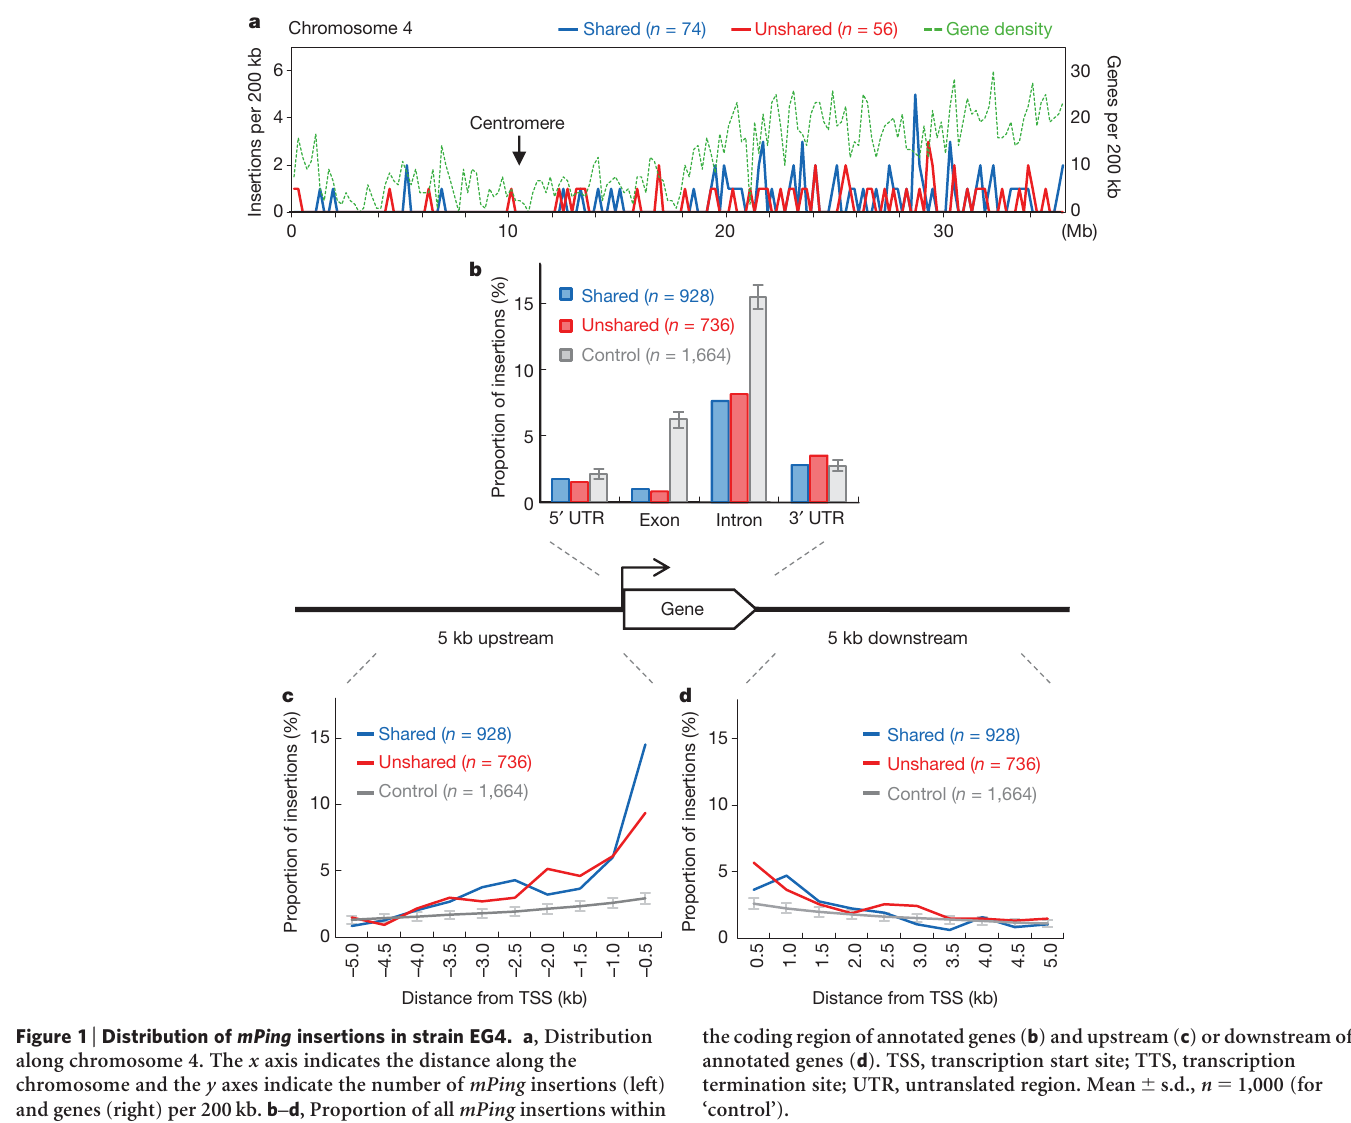
\includegraphics[width=\textwidth]{naito-transposons-2009-fig1}
        \caption{Naito (2009) \cite{naito_unexpected_2009}}
      \end{figure}

      \begin{figure}[h!]
        \centering
        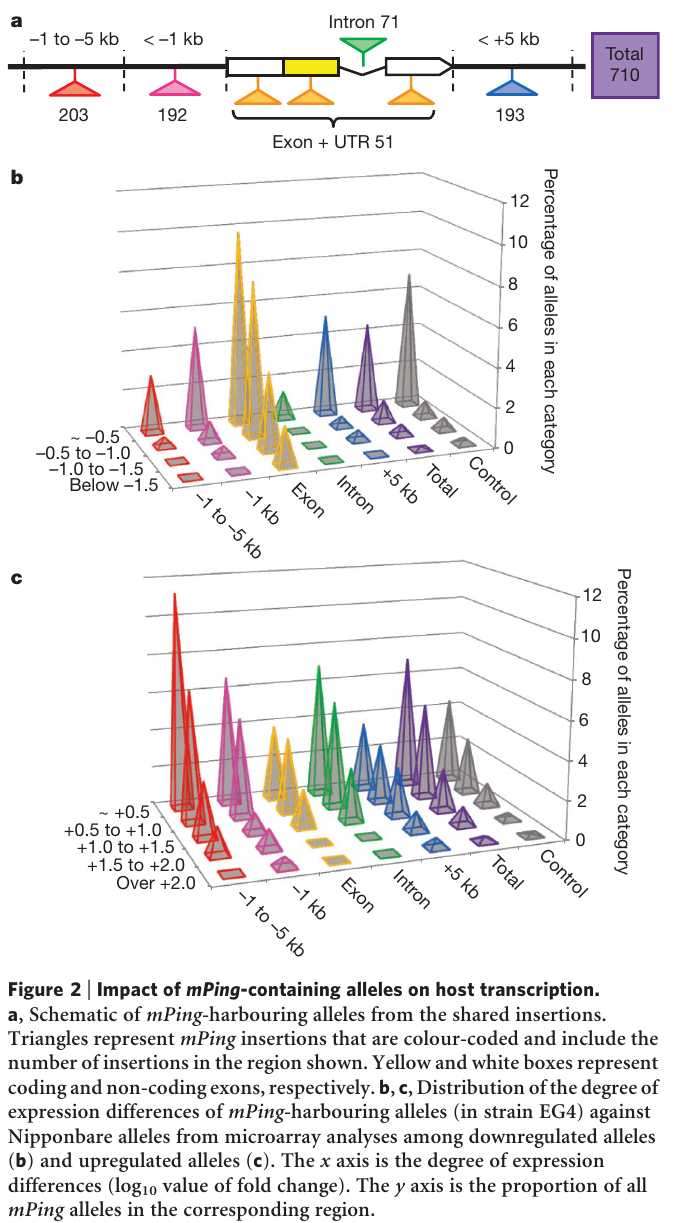
\includegraphics[height=0.7\textheight]{naito-transposons-2009-fig2}
        \caption{Naito (2009) \cite{naito_unexpected_2009}}
      \end{figure}
      \FloatBarrier

    \subsubsection{Haudry (2013) An atlas of over 90,000 conserved
    noncoding sequences provides insight into crucifer regulatory regions}

      Citation \cite{haudry_atlas_2013}

      They sequence three new crucifers: \textit{Leavenworthia alabamica},
      \textit{Sisymbrium irio} and \textit{Aethionema arabicum}.

      Performs an alignment of 9 Brassicaceae genomes, identifying
      conserved regions.


